\section{Resultat}
Denna del av dokumentet presenterar resultatet av vårt arbete.
Här kommer vi diskutera både hur systemet ser ut och används, samt hur
det är uppbyggt rent tekniskt.

\subsection{Översikt av systemet}
Det finns två huvuddelar i systemet. Handböckerna och kartoteket.

Handböckerna beskriver hur man förbereder olika typer av operationer.
Varje handbok har en lista med artiklar som behövs till operationen, en så kallad plocklista.
Artiklarna är kopplade till kartoteket, som bland annat innehåller information om var i förråden artiklarna finns placerade.

När en patient registreras skapas en instans av en handbok.
I denna instans kan man checka av en lista med artiklar som ska användas under operationen och även andra förberedelser.
En samordnare kan se en översikt på hur långt man har kommit med de förberedelserna för varje instans.
Se en översikt i figur \ref{fig:overview}.

\begin{figure}
  \centering
  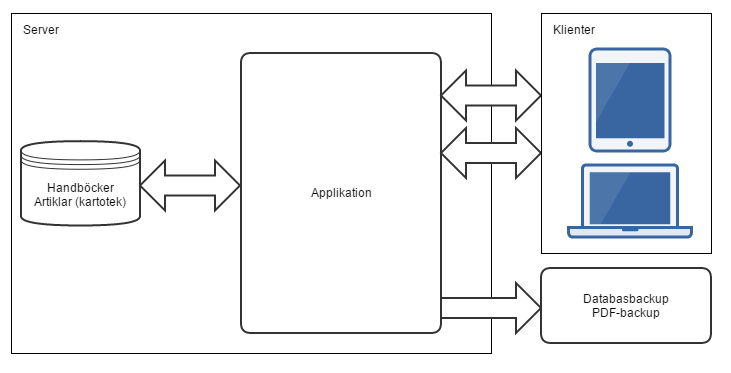
\includegraphics[width=0.9\textwidth]{images/overview.png}
  \caption{Översikt av systemet}
  \label{fig:overview}
\end{figure}

\subsubsection{Server och klient}
Applikationen består av en server som distribuerar en hemsida till flera klienter.
Servern kan köras i en Windowsmiljö.
Hemsidan är responsiv och fungerar på surfplattor och datorer i olika format.

\subsubsection{Kartoteket}
I kartoteket finns information om alla artiklar som Region Östergötland har i förråden.
Här finns bland annat information om var artiklarna är placerade samt information relaterade till inköp av artiklar.

Läs mer om kartoteket i "Kartoteket" nedan.

\subsection{Tekniker}
Vi börjar med att beskriva tekniken bakom systemet.

\subsubsection{Översikt}
Programmet är uppdelat i två delar, en serverdel och en klientdel.
Serverdelen består av databaskopplingar som kopplas ihop och distribueras ut genom hemsidor till klienterna.

\begin{figure}
  \centering
  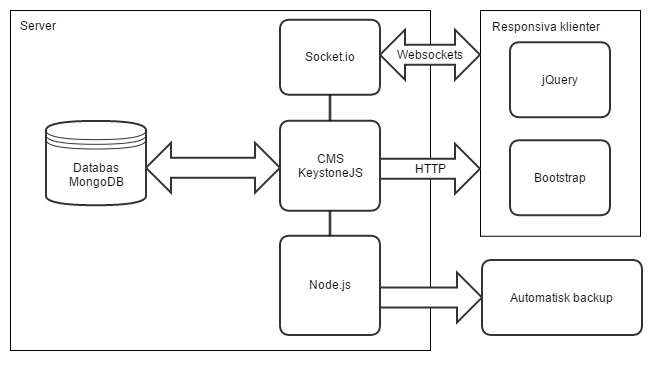
\includegraphics[width=0.9\textwidth]{images/techoverview.png}
  \caption{En översikt över tekniken}
  \label{fig:techoverview}
\end{figure}

I figur \ref{fig:techoverview} kan man se en översikt över de mest betydelsefulla tekniker och bibliotek som används för att bygga upp programmet.

\subsubsection{Back-end}
Koden till servern har skrivits helt i javascript.
Dels för att underlätta inlärningskurvan genom att använda samma språk som på klienten och dels för att realtidskommunikation mellan klienterna underlättas.
Grunden till programmet är node.js vilket är en plattform för att utveckla självständiga program i javascript med inbyggd pakethanterare.
Pakethanteraren gör det enkelt att installera externa bibliotek.

Det största och mest betydelsefulla ramverket för detta projekt är KeystoneJS, ett CMS-ramverk till node.js.
Följande är några punkter KeystoneJS underlättar:
\begin{itemize}
  \item Hjälper till att abstrahera systemet. Se avsnittet om MVC nedan.
  \item Skapar automatiskt en administreringssida för varje databasmodell.
    Huvuddelen av administeringen har dock bytts ut då den automatgenererade kan vara något begränsad.
  \item Har ett inbyggt användarsystem som är lätt att modifiera och byta ut.
  \item Sköter all kommunikation över http-protokollet till klienterna, dvs. gör hemsidan åtkomlig.
  \item Har inbyggt stöd för templatespråk som exempelvis Handlebars\footnote{TODO: bättre referens. http://handlebarsjs.com/ (2015-04-18)} och Less\footnote{TODO: Bättre referens. http://lesscss.org/ (2015-04-18)}.
\end{itemize}

För realtidskommunikation används ett programmeringsinterface vid namn socket.io\footnote{TODO: bättre referens. http://socket.io/ (2015-04-18)} användas.
Det är väldigt smidigt eftersom det väljer automatiskt hur datan ska skickas beroende på vilken webbläsare som används och vad den stödjer.
Socket.io är event-baserat vilket betyder att man skapar events på antingen klient eller serversida som man sedan kan trigga från motsatt sida.
Vanliga javascript-object kan skickas tillsammans med eventen.

\subsubsection{Front-end}




%\subsection{Gruppens gemensamma erfarenheter}
%\subsection{Översikt över de inviduella utredningarna}
